\pgfdeclareplotmark{cross} {
\pgfpathmoveto{\pgfpoint{-0.3\pgfplotmarksize}{\pgfplotmarksize}}
\pgfpathlineto{\pgfpoint{+0.3\pgfplotmarksize}{\pgfplotmarksize}}
\pgfpathlineto{\pgfpoint{+0.3\pgfplotmarksize}{0.3\pgfplotmarksize}}
\pgfpathlineto{\pgfpoint{+1\pgfplotmarksize}{0.3\pgfplotmarksize}}
\pgfpathlineto{\pgfpoint{+1\pgfplotmarksize}{-0.3\pgfplotmarksize}}
\pgfpathlineto{\pgfpoint{+0.3\pgfplotmarksize}{-0.3\pgfplotmarksize}}
\pgfpathlineto{\pgfpoint{+0.3\pgfplotmarksize}{-1.\pgfplotmarksize}}
\pgfpathlineto{\pgfpoint{-0.3\pgfplotmarksize}{-1.\pgfplotmarksize}}
\pgfpathlineto{\pgfpoint{-0.3\pgfplotmarksize}{-0.3\pgfplotmarksize}}
\pgfpathlineto{\pgfpoint{-1.\pgfplotmarksize}{-0.3\pgfplotmarksize}}
\pgfpathlineto{\pgfpoint{-1.\pgfplotmarksize}{0.3\pgfplotmarksize}}
\pgfpathlineto{\pgfpoint{-0.3\pgfplotmarksize}{0.3\pgfplotmarksize}}
\pgfpathclose
\pgfusepathqstroke
}
\pgfdeclareplotmark{cross*} {
\pgfpathmoveto{\pgfpoint{-0.3\pgfplotmarksize}{\pgfplotmarksize}}
\pgfpathlineto{\pgfpoint{+0.3\pgfplotmarksize}{\pgfplotmarksize}}
\pgfpathlineto{\pgfpoint{+0.3\pgfplotmarksize}{0.3\pgfplotmarksize}}
\pgfpathlineto{\pgfpoint{+1\pgfplotmarksize}{0.3\pgfplotmarksize}}
\pgfpathlineto{\pgfpoint{+1\pgfplotmarksize}{-0.3\pgfplotmarksize}}
\pgfpathlineto{\pgfpoint{+0.3\pgfplotmarksize}{-0.3\pgfplotmarksize}}
\pgfpathlineto{\pgfpoint{+0.3\pgfplotmarksize}{-1.\pgfplotmarksize}}
\pgfpathlineto{\pgfpoint{-0.3\pgfplotmarksize}{-1.\pgfplotmarksize}}
\pgfpathlineto{\pgfpoint{-0.3\pgfplotmarksize}{-0.3\pgfplotmarksize}}
\pgfpathlineto{\pgfpoint{-1.\pgfplotmarksize}{-0.3\pgfplotmarksize}}
\pgfpathlineto{\pgfpoint{-1.\pgfplotmarksize}{0.3\pgfplotmarksize}}
\pgfpathlineto{\pgfpoint{-0.3\pgfplotmarksize}{0.3\pgfplotmarksize}}
\pgfpathclose
\pgfusepathqfillstroke
}
\pgfdeclareplotmark{newstar} {
\pgfpathmoveto{\pgfqpoint{0pt}{\pgfplotmarksize}}
\pgfpathlineto{\pgfqpointpolar{44}{0.5\pgfplotmarksize}}
\pgfpathlineto{\pgfqpointpolar{18}{\pgfplotmarksize}}
\pgfpathlineto{\pgfqpointpolar{-20}{0.5\pgfplotmarksize}}
\pgfpathlineto{\pgfqpointpolar{-54}{\pgfplotmarksize}}
\pgfpathlineto{\pgfqpointpolar{-90}{0.5\pgfplotmarksize}}
\pgfpathlineto{\pgfqpointpolar{234}{\pgfplotmarksize}}
\pgfpathlineto{\pgfqpointpolar{198}{0.5\pgfplotmarksize}}
\pgfpathlineto{\pgfqpointpolar{162}{\pgfplotmarksize}}
\pgfpathlineto{\pgfqpointpolar{134}{0.5\pgfplotmarksize}}
\pgfpathclose
\pgfusepathqstroke
}
\pgfdeclareplotmark{newstar*} {
\pgfpathmoveto{\pgfqpoint{0pt}{\pgfplotmarksize}}
\pgfpathlineto{\pgfqpointpolar{44}{0.5\pgfplotmarksize}}
\pgfpathlineto{\pgfqpointpolar{18}{\pgfplotmarksize}}
\pgfpathlineto{\pgfqpointpolar{-20}{0.5\pgfplotmarksize}}
\pgfpathlineto{\pgfqpointpolar{-54}{\pgfplotmarksize}}
\pgfpathlineto{\pgfqpointpolar{-90}{0.5\pgfplotmarksize}}
\pgfpathlineto{\pgfqpointpolar{234}{\pgfplotmarksize}}
\pgfpathlineto{\pgfqpointpolar{198}{0.5\pgfplotmarksize}}
\pgfpathlineto{\pgfqpointpolar{162}{\pgfplotmarksize}}
\pgfpathlineto{\pgfqpointpolar{134}{0.5\pgfplotmarksize}}
\pgfpathclose
\pgfusepathqfillstroke
}
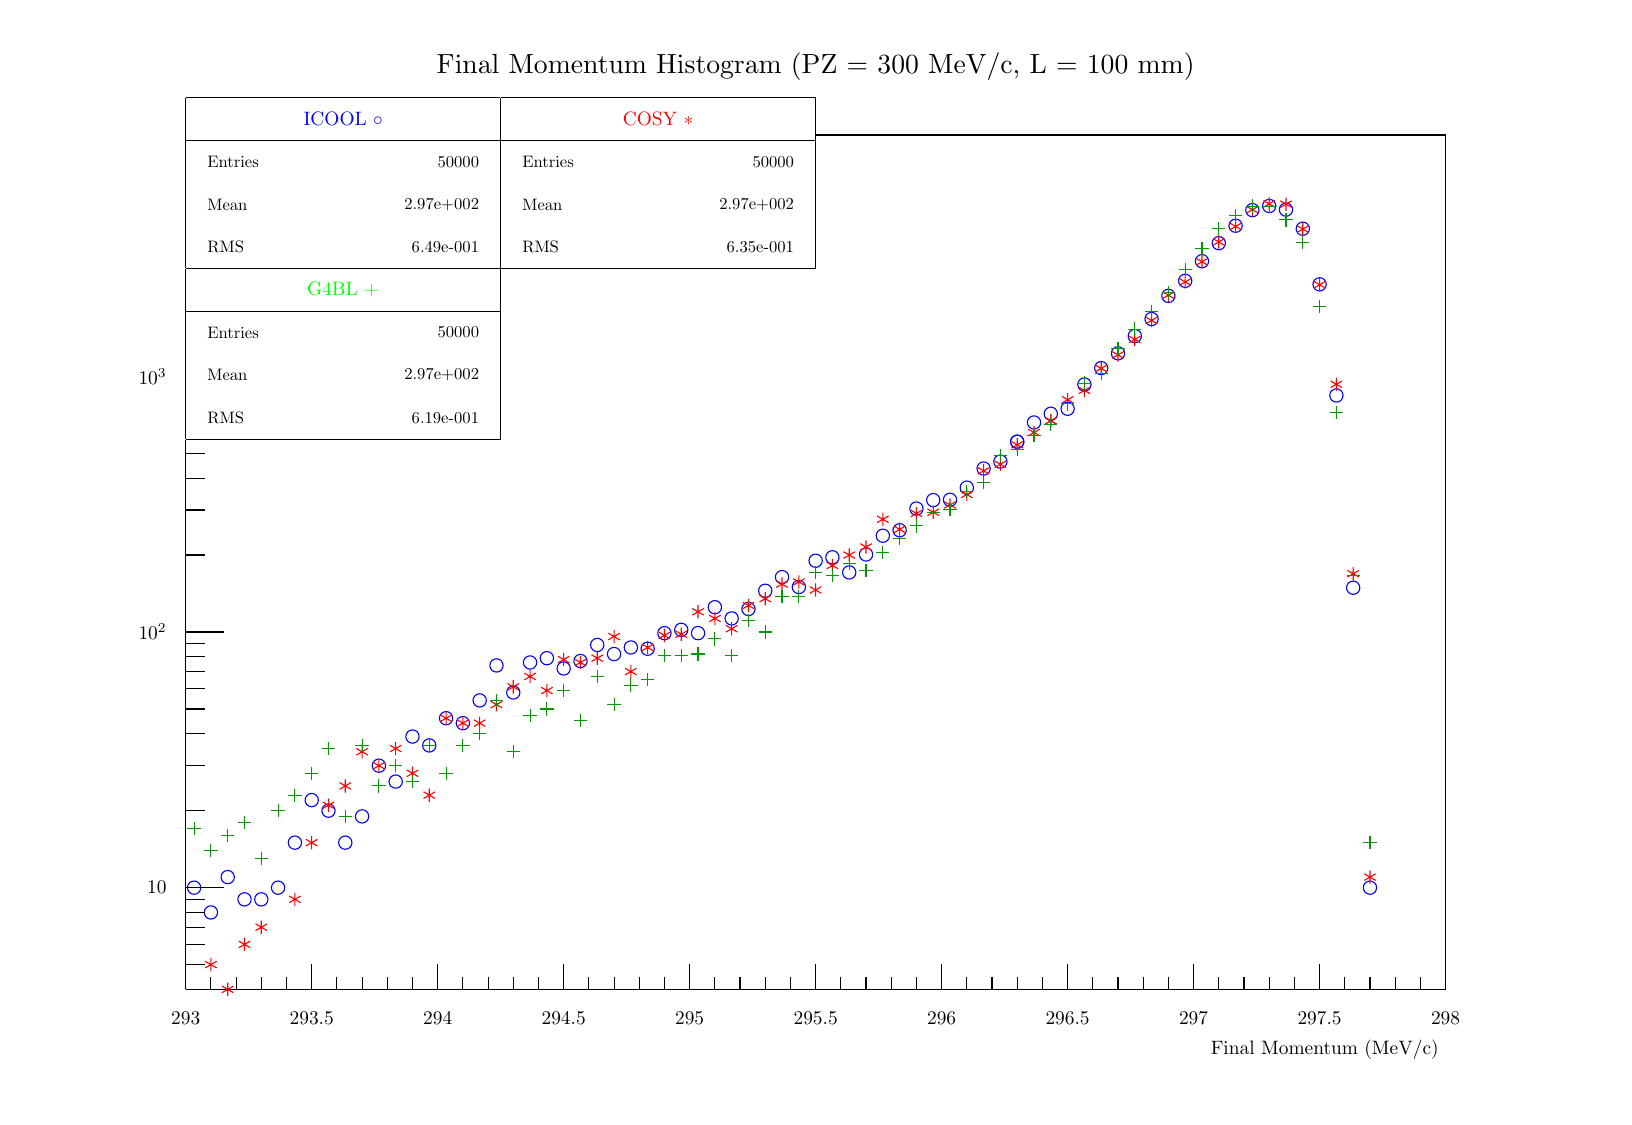
\begin{tikzpicture}
\definecolor{c}{rgb}{1,1,1};
\draw [color=c, fill=c] (0,0) rectangle (20,13.5632);
\draw [color=c, fill=c] (2,1.35632) rectangle (18,12.2069);
\definecolor{c}{rgb}{0,0,0};
\draw [c] (2,1.35632) -- (2,12.2069) -- (18,12.2069) -- (18,1.35632) -- (2,1.35632);
\definecolor{c}{rgb}{1,1,1};
\draw [color=c, fill=c] (2,1.35632) rectangle (18,12.2069);
\definecolor{c}{rgb}{0,0,0};
\draw [c] (2,1.35632) -- (2,12.2069) -- (18,12.2069) -- (18,1.35632) -- (2,1.35632);
\definecolor{c}{rgb}{0,0,1};
\foreach \P in
 {(2.10667,2.64836),(2.32,2.33371),(2.53333,2.78275),(2.74667,2.49979),(2.96,2.49979),(3.17333,2.64836),(3.38667,3.2201),(3.6,3.76014),(3.81333,3.62575),(4.02667,3.2201),(4.24,3.55342),(4.45333,4.19748),(4.66667,3.9957),(4.88,4.56744),(5.09333,4.4545
7),(5.30667,4.80021),(5.52,4.73753),(5.73333,5.02631),(5.94667,5.47059),(6.16,5.12707),(6.37333,5.5082),(6.58667,5.56279),(6.8,5.43196),(7.01333,5.52663),(7.22667,5.73085),(7.44,5.61534),(7.65333,5.6988),(7.86667,5.6825),(8.08,5.881),(8.29333,5.9231)
,(8.50667,5.881),(8.72,6.20982),(8.93333,6.06751),(9.14667,6.18708),(9.36,6.41911),(9.57333,6.59273),(9.78667,6.46691),(10,6.80024),(10.2133,6.84408),(10.4267,6.65167),(10.64,6.8796),(10.8533,7.11785),(11.0667,7.18721),(11.28,7.46298),(11.4933,7.5701
2),(11.7067,7.57441),(11.92,7.72854),(12.1333,7.97147),(12.3467,8.05924),(12.56,8.31176)}{\draw[mark options={color=c,fill=c},mark size=2.402402pt,mark=o] plot coordinates {\P};}
\foreach \P in
 {(12.56,8.31176),(12.7733,8.55608),(12.9867,8.66698),(13.2,8.73069),(13.4133,9.03814),(13.6267,9.24659),(13.84,9.43504),(14.0533,9.65322),(14.2667,9.87017),(14.48,10.1645),(14.6933,10.3552),(14.9067,10.6044),(15.12,10.8336),(15.3333,11.0545),(15.546
7,11.2525),(15.76,11.3057),(15.9733,11.2588),(16.1867,11.017),(16.4,10.3109),(16.6133,8.89949),(16.8267,6.45748),(17.04,2.64836)}{\draw[mark options={color=c,fill=c},mark size=2.402402pt,mark=o] plot coordinates {\P};}
\definecolor{c}{rgb}{1,1,1};
\draw [color=c, fill=c] (2,10.5115) rectangle (6,12.6816);
\definecolor{c}{rgb}{0,0,0};
\draw [c] (2,10.5115) -- (6,10.5115);
\draw [c] (6,10.5115) -- (6,12.6816);
\draw [c] (6,12.6816) -- (2,12.6816);
\draw [c] (2,12.6816) -- (2,10.5115);
\draw[color=blue](4,12.4103) node[scale=0.7, rotate=0]{ICOOL $\circ$};
\draw [c] (2,12.1391) -- (6,12.1391);
\draw [anchor= west] (2.2,11.8678) node[scale=0.6, rotate=0]{Entries };
\draw [anchor= east] (5.8,11.8678) node[scale=0.6, rotate=0]{ 50000};
\draw [anchor= west] (2.2,11.3253) node[scale=0.6, rotate=0]{Mean  };
\draw [anchor= east] (5.8,11.3253) node[scale=0.6, rotate=0]{ 2.97e+002};
\draw [anchor= west] (2.2,10.7828) node[scale=0.6, rotate=0]{RMS   };
\draw [anchor= east] (5.8,10.7828) node[scale=0.6, rotate=0]{ 6.49e-001};
\draw [c] (2,1.35632) -- (18,1.35632);
\draw [anchor= east] (18,0.596782) node[scale=0.7, rotate=0]{Final Momentum (MeV/c)};
\draw [c] (2,1.68184) -- (2,1.35632);
\draw [c] (2.32,1.51908) -- (2.32,1.35632);
\draw [c] (2.64,1.51908) -- (2.64,1.35632);
\draw [c] (2.96,1.51908) -- (2.96,1.35632);
\draw [c] (3.28,1.51908) -- (3.28,1.35632);
\draw [c] (3.6,1.68184) -- (3.6,1.35632);
\draw [c] (3.92,1.51908) -- (3.92,1.35632);
\draw [c] (4.24,1.51908) -- (4.24,1.35632);
\draw [c] (4.56,1.51908) -- (4.56,1.35632);
\draw [c] (4.88,1.51908) -- (4.88,1.35632);
\draw [c] (5.2,1.68184) -- (5.2,1.35632);
\draw [c] (5.52,1.51908) -- (5.52,1.35632);
\draw [c] (5.84,1.51908) -- (5.84,1.35632);
\draw [c] (6.16,1.51908) -- (6.16,1.35632);
\draw [c] (6.48,1.51908) -- (6.48,1.35632);
\draw [c] (6.8,1.68184) -- (6.8,1.35632);
\draw [c] (7.12,1.51908) -- (7.12,1.35632);
\draw [c] (7.44,1.51908) -- (7.44,1.35632);
\draw [c] (7.76,1.51908) -- (7.76,1.35632);
\draw [c] (8.08,1.51908) -- (8.08,1.35632);
\draw [c] (8.4,1.68184) -- (8.4,1.35632);
\draw [c] (8.72,1.51908) -- (8.72,1.35632);
\draw [c] (9.04,1.51908) -- (9.04,1.35632);
\draw [c] (9.36,1.51908) -- (9.36,1.35632);
\draw [c] (9.68,1.51908) -- (9.68,1.35632);
\draw [c] (10,1.68184) -- (10,1.35632);
\draw [c] (10.32,1.51908) -- (10.32,1.35632);
\draw [c] (10.64,1.51908) -- (10.64,1.35632);
\draw [c] (10.96,1.51908) -- (10.96,1.35632);
\draw [c] (11.28,1.51908) -- (11.28,1.35632);
\draw [c] (11.6,1.68184) -- (11.6,1.35632);
\draw [c] (11.92,1.51908) -- (11.92,1.35632);
\draw [c] (12.24,1.51908) -- (12.24,1.35632);
\draw [c] (12.56,1.51908) -- (12.56,1.35632);
\draw [c] (12.88,1.51908) -- (12.88,1.35632);
\draw [c] (13.2,1.68184) -- (13.2,1.35632);
\draw [c] (13.52,1.51908) -- (13.52,1.35632);
\draw [c] (13.84,1.51908) -- (13.84,1.35632);
\draw [c] (14.16,1.51908) -- (14.16,1.35632);
\draw [c] (14.48,1.51908) -- (14.48,1.35632);
\draw [c] (14.8,1.68184) -- (14.8,1.35632);
\draw [c] (15.12,1.51908) -- (15.12,1.35632);
\draw [c] (15.44,1.51908) -- (15.44,1.35632);
\draw [c] (15.76,1.51908) -- (15.76,1.35632);
\draw [c] (16.08,1.51908) -- (16.08,1.35632);
\draw [c] (16.4,1.68184) -- (16.4,1.35632);
\draw [c] (16.72,1.51908) -- (16.72,1.35632);
\draw [c] (17.04,1.51908) -- (17.04,1.35632);
\draw [c] (17.36,1.51908) -- (17.36,1.35632);
\draw [c] (17.68,1.51908) -- (17.68,1.35632);
\draw [c] (18,1.68184) -- (18,1.35632);
\draw [anchor=base] (2,0.908736) node[scale=0.7, rotate=0]{293};
\draw [anchor=base] (3.6,0.908736) node[scale=0.7, rotate=0]{293.5};
\draw [anchor=base] (5.2,0.908736) node[scale=0.7, rotate=0]{294};
\draw [anchor=base] (6.8,0.908736) node[scale=0.7, rotate=0]{294.5};
\draw [anchor=base] (8.4,0.908736) node[scale=0.7, rotate=0]{295};
\draw [anchor=base] (10,0.908736) node[scale=0.7, rotate=0]{295.5};
\draw [anchor=base] (11.6,0.908736) node[scale=0.7, rotate=0]{296};
\draw [anchor=base] (13.2,0.908736) node[scale=0.7, rotate=0]{296.5};
\draw [anchor=base] (14.8,0.908736) node[scale=0.7, rotate=0]{297};
\draw [anchor=base] (16.4,0.908736) node[scale=0.7, rotate=0]{297.5};
\draw [anchor=base] (18,0.908736) node[scale=0.7, rotate=0]{298};
\draw [c] (2,1.35632) -- (2,12.2069);
\draw [c] (2.24,1.67097) -- (2,1.67097);
\draw [c] (2.24,1.92805) -- (2,1.92805);
\draw [c] (2.24,2.14542) -- (2,2.14542);
\draw [c] (2.24,2.33371) -- (2,2.33371);
\draw [c] (2.24,2.49979) -- (2,2.49979);
\draw [c] (2.48,2.64836) -- (2,2.64836);
\draw [anchor= east] (1.844,2.64836) node[scale=0.7, rotate=0]{10};
\draw [c] (2.24,3.62575) -- (2,3.62575);
\draw [c] (2.24,4.19748) -- (2,4.19748);
\draw [c] (2.24,4.60313) -- (2,4.60313);
\draw [c] (2.24,4.91778) -- (2,4.91778);
\draw [c] (2.24,5.17487) -- (2,5.17487);
\draw [c] (2.24,5.39223) -- (2,5.39223);
\draw [c] (2.24,5.58052) -- (2,5.58052);
\draw [c] (2.24,5.74661) -- (2,5.74661);
\draw [c] (2.48,5.89517) -- (2,5.89517);
\draw [anchor= east] (1.844,5.89517) node[scale=0.7, rotate=0]{$10^{2}$};
\draw [c] (2.24,6.87256) -- (2,6.87256);
\draw [c] (2.24,7.4443) -- (2,7.4443);
\draw [c] (2.24,7.84995) -- (2,7.84995);
\draw [c] (2.24,8.1646) -- (2,8.1646);
\draw [c] (2.24,8.42169) -- (2,8.42169);
\draw [c] (2.24,8.63905) -- (2,8.63905);
\draw [c] (2.24,8.82734) -- (2,8.82734);
\draw [c] (2.24,8.99342) -- (2,8.99342);
\draw [c] (2.48,9.14199) -- (2,9.14199);
\draw [anchor= east] (1.844,9.14199) node[scale=0.7, rotate=0]{$10^{3}$};
\draw [c] (2.24,10.1194) -- (2,10.1194);
\draw [c] (2.24,10.6911) -- (2,10.6911);
\draw [c] (2.24,11.0968) -- (2,11.0968);
\draw [c] (2.24,11.4114) -- (2,11.4114);
\draw [c] (2.24,11.6685) -- (2,11.6685);
\draw [c] (2.24,11.8859) -- (2,11.8859);
\draw [c] (2.24,12.0742) -- (2,12.0742);
\definecolor{c}{rgb}{1,1,1};
\draw [color=c, fill=c] (2,10.5115) rectangle (6,12.6816);
\definecolor{c}{rgb}{0,0,0};
\draw [c] (2,10.5115) -- (6,10.5115);
\draw [c] (6,10.5115) -- (6,12.6816);
\draw [c] (6,12.6816) -- (2,12.6816);
\draw [c] (2,12.6816) -- (2,10.5115);
\draw[color=blue](4,12.4103) node[scale=0.7, rotate=0]{ICOOL $\circ$};
\draw [c] (2,12.1391) -- (6,12.1391);
\draw [anchor= west] (2.2,11.8678) node[scale=0.6, rotate=0]{Entries };
\draw [anchor= east] (5.8,11.8678) node[scale=0.6, rotate=0]{ 50000};
\draw [anchor= west] (2.2,11.3253) node[scale=0.6, rotate=0]{Mean  };
\draw [anchor= east] (5.8,11.3253) node[scale=0.6, rotate=0]{ 2.97e+002};
\draw [anchor= west] (2.2,10.7828) node[scale=0.6, rotate=0]{RMS   };
\draw [anchor= east] (5.8,10.7828) node[scale=0.6, rotate=0]{ 6.49e-001};
\draw (10,13.0816) node[scale=1, rotate=0]{Final Momentum Histogram (PZ = 300 MeV/c, L = 100 mm)};
\definecolor{c}{rgb}{1,0,0};
\foreach \P in
 {(2.32,1.67097),(2.53333,1.35632),(2.74667,1.92806),(2.96,2.14542),(3.38667,2.49979),(3.6,3.2201),(3.81333,3.69455),(4.02667,3.9404),(4.24,4.37397),(4.45333,4.19748),(4.66667,4.41485),(4.88,4.1002),(5.09333,3.82282),(5.30667,4.80021),(5.52,4.73753),
(5.73333,4.73753),(5.94667,4.97309),(6.16,5.19818),(6.37333,5.33047),(6.58667,5.15117),(6.8,5.54483),(7.01333,5.5082),(7.22667,5.56279),(7.44,5.83761),(7.65333,5.39224),(7.86667,5.6988),(8.08,5.85222),(8.29333,5.86669),(8.50667,6.15226),(8.72,6.06751
),(8.93333,5.93685),(9.14667,6.23221),(9.36,6.31834),(9.57333,6.50402),(9.78667,6.53122),(10,6.4288),(10.2133,6.73958),(10.4267,6.87256),(10.64,6.97454),(10.8533,7.32673),(11.0667,7.19845),(11.28,7.40135),(11.4933,7.41581),(11.7067,7.50861),(11.92,7.
64137),(12.1333,7.94206),(12.3467,8.0254),(12.56,8.27312),(12.7733,8.42872),(12.9867,8.57729)}{\draw[mark options={color=c,fill=c},mark size=2.402402pt,mark=asterisk] plot coordinates {\P};}
\foreach \P in
 {(12.9867,8.57729),(13.2,8.84486),(13.4133,8.96334),(13.6267,9.24265),(13.84,9.41427),(14.0533,9.61139),(14.2667,9.85153),(14.48,10.172),(14.6933,10.3408),(14.9067,10.5968),(15.12,10.8484),(15.3333,11.0458),(15.5467,11.2585),(15.76,11.3325),(15.9733
,11.3284),(16.1867,11.0118),(16.4,10.3054),(16.6133,9.04117),(16.8267,6.63508),(17.04,2.78275)}{\draw[mark options={color=c,fill=c},mark size=2.402402pt,mark=asterisk] plot coordinates {\P};}
\definecolor{c}{rgb}{1,1,1};
\draw [color=c, fill=c] (6,10.5115) rectangle (10,12.6816);
\definecolor{c}{rgb}{0,0,0};
\draw [c] (6,10.5115) -- (10,10.5115);
\draw [c] (10,10.5115) -- (10,12.6816);
\draw [c] (10,12.6816) -- (6,12.6816);
\draw [c] (6,12.6816) -- (6,10.5115);
\draw [color=red](8,12.4103) node[scale=0.7, rotate=0]{COSY $*$};
\draw [c] (6,12.1391) -- (10,12.1391);
\draw [anchor= west] (6.2,11.8678) node[scale=0.6, rotate=0]{Entries };
\draw [anchor= east] (9.8,11.8678) node[scale=0.6, rotate=0]{ 50000};
\draw [anchor= west] (6.2,11.3253) node[scale=0.6, rotate=0]{Mean  };
\draw [anchor= east] (9.8,11.3253) node[scale=0.6, rotate=0]{ 2.97e+002};
\draw [anchor= west] (6.2,10.7828) node[scale=0.6, rotate=0]{RMS   };
\draw [anchor= east] (9.8,10.7828) node[scale=0.6, rotate=0]{ 6.35e-001};
\definecolor{c}{rgb}{1,1,1};
\draw [color=c, fill=c] (6,10.5115) rectangle (10,12.6816);
\definecolor{c}{rgb}{0,0,0};
\draw [c] (6,10.5115) -- (10,10.5115);
\draw [c] (10,10.5115) -- (10,12.6816);
\draw [c] (10,12.6816) -- (6,12.6816);
\draw [c] (6,12.6816) -- (6,10.5115);
\draw [color=red](8,12.4103) node[scale=0.7, rotate=0]{COSY $*$};
\draw [c] (6,12.1391) -- (10,12.1391);
\draw [anchor= west] (6.2,11.8678) node[scale=0.6, rotate=0]{Entries };
\draw [anchor= east] (9.8,11.8678) node[scale=0.6, rotate=0]{ 50000};
\draw [anchor= west] (6.2,11.3253) node[scale=0.6, rotate=0]{Mean  };
\draw [anchor= east] (9.8,11.3253) node[scale=0.6, rotate=0]{ 2.97e+002};
\draw [anchor= west] (6.2,10.7828) node[scale=0.6, rotate=0]{RMS   };
\draw [anchor= east] (9.8,10.7828) node[scale=0.6, rotate=0]{ 6.35e-001};
\definecolor{c}{rgb}{0,0.6,0};
\foreach \P in
 {(2.10667,3.39658),(2.32,3.12281),(2.53333,3.3111),(2.74667,3.47718),(2.96,3.01831),(3.17333,3.62575),(3.38667,3.82282),(3.6,4.1002),(3.81333,4.41485),(4.02667,3.55342),(4.24,4.45457),(4.45333,3.9404),(4.66667,4.19748),(4.88,3.9957),(5.09333,4.45457
),(5.30667,4.1002),(5.52,4.45457),(5.73333,4.60314),(5.94667,5.02631),(6.16,4.37397),(6.37333,4.83054),(6.58667,4.91779),(6.8,5.15117),(7.01333,4.76922),(7.22667,5.33047),(7.44,4.97309),(7.65333,5.22111),(7.86667,5.28774),(8.08,5.59804),(8.29333,5.59
804),(8.50667,5.61534),(8.72,5.80793),(8.93333,5.59804),(9.14667,6.04233),(9.36,5.89517),(9.57333,6.34934),(9.78667,6.34934),(10,6.65167),(10.2133,6.60982),(10.4267,6.77023),(10.64,6.67619),(10.8533,6.90049),(11.0667,7.08791),(11.28,7.24252),(11.4933
,7.41101),(11.7067,7.44899),(11.92,7.68166),(12.1333,7.79239),(12.3467,8.13323),(12.56,8.21175)}{\draw[mark options={color=c,fill=c},mark size=2.402402pt,mark=+] plot coordinates {\P};}
\foreach \P in
 {(12.56,8.21175),(12.7733,8.3908),(12.9867,8.53455),(13.2,8.79164),(13.4133,9.05624),(13.6267,9.17681),(13.84,9.49338),(14.0533,9.74165),(14.2667,9.96217),(14.48,10.2095),(14.6933,10.4947),(14.9067,10.7666),(15.12,11.0189),(15.3333,11.1816),(15.5467
,11.3045),(15.76,11.3036),(15.9733,11.1288),(16.1867,10.84),(16.4,10.0299),(16.6133,8.68073),(16.8267,6.60982),(17.04,3.2201)}{\draw[mark options={color=c,fill=c},mark size=2.402402pt,mark=+] plot coordinates {\P};}
\definecolor{c}{rgb}{1,1,1};
\draw [color=c, fill=c] (2,8.34138) rectangle (6,10.5115);
\definecolor{c}{rgb}{0,0,0};
\draw [c] (2,8.34138) -- (6,8.34138);
\draw [c] (6,8.34138) -- (6,10.5115);
\draw [c] (6,10.5115) -- (2,10.5115);
\draw [c] (2,10.5115) -- (2,8.34138);
\draw [color=green](4,10.2402) node[scale=0.7, rotate=0]{G4BL $+$};
\draw [c] (2,9.96897) -- (6,9.96897);
\draw [anchor= west] (2.2,9.6977) node[scale=0.6, rotate=0]{Entries };
\draw [anchor= east] (5.8,9.6977) node[scale=0.6, rotate=0]{ 50000};
\draw [anchor= west] (2.2,9.15517) node[scale=0.6, rotate=0]{Mean  };
\draw [anchor= east] (5.8,9.15517) node[scale=0.6, rotate=0]{ 2.97e+002};
\draw [anchor= west] (2.2,8.61264) node[scale=0.6, rotate=0]{RMS   };
\draw [anchor= east] (5.8,8.61264) node[scale=0.6, rotate=0]{ 6.19e-001};
\definecolor{c}{rgb}{1,1,1};
\draw [color=c, fill=c] (2,8.34138) rectangle (6,10.5115);
\definecolor{c}{rgb}{0,0,0};
\draw [c] (2,8.34138) -- (6,8.34138);
\draw [c] (6,8.34138) -- (6,10.5115);
\draw [c] (6,10.5115) -- (2,10.5115);
\draw [c] (2,10.5115) -- (2,8.34138);
\draw [color=green](4,10.2402) node[scale=0.7, rotate=0]{G4BL $+$};
\draw [c] (2,9.96897) -- (6,9.96897);
\draw [anchor= west] (2.2,9.6977) node[scale=0.6, rotate=0]{Entries };
\draw [anchor= east] (5.8,9.6977) node[scale=0.6, rotate=0]{ 50000};
\draw [anchor= west] (2.2,9.15517) node[scale=0.6, rotate=0]{Mean  };
\draw [anchor= east] (5.8,9.15517) node[scale=0.6, rotate=0]{ 2.97e+002};
\draw [anchor= west] (2.2,8.61264) node[scale=0.6, rotate=0]{RMS   };
\draw [anchor= east] (5.8,8.61264) node[scale=0.6, rotate=0]{ 6.19e-001};
\end{tikzpicture}
